%\begin{figure}[h]
	%\centering
	%\missingfigure{Komponentendiagramm}		
	%\caption{Komponentendiagramm - A}
	%\label{fig:komponentendiagramm-a}
%\end{figure}

%\begin{tcolorbox}
%Die strukturelle Übersicht des zu entwickelnden Systems wird mittels Komponentendiagrammen modelliert. 
%Auf jedes Diagramm muss eine textuelle Beschreibung (Fließtext mit Umbrüchen / Absätzen oder Tabelle) folgen, in der die Aufgaben der %Subkomponenten beschrieben werden. 
%\end{tcolorbox}

\section{Backend}

\begin{figure}[H]
	\centering
	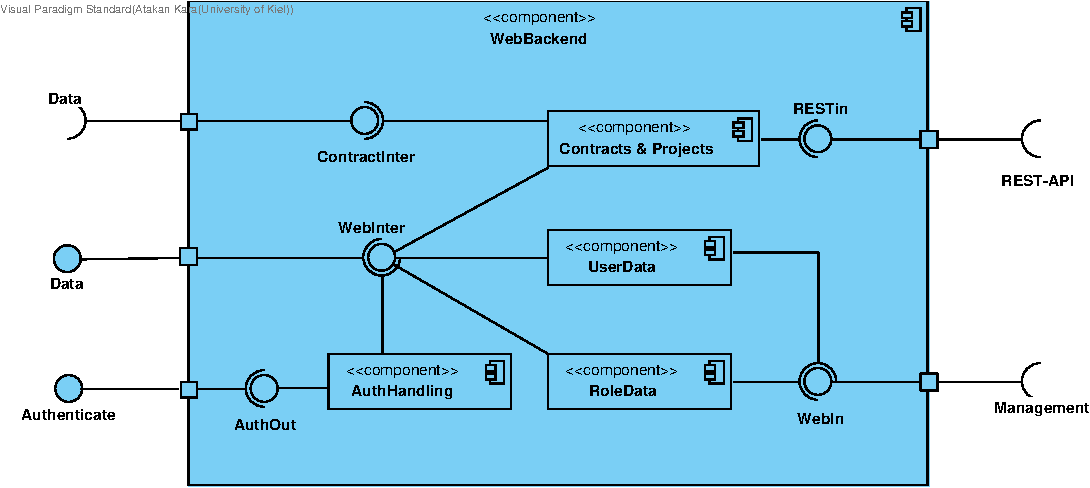
\includegraphics[width=16cm]{img/diagrams/cp_backend.pdf}	
	\caption{Komponentendiagramm - Backend}
	\label{fig:komponentendiagramm-backend}
\end{figure}

\begin{longtable}[h]{|p{2.5cm}|p{10.0cm}|}
	\caption{Tabelle - Komponentendiagramm-Backend}
	\centering
	\label{tab:table_comp_backend}
	\endlastfoot
	\hline \multicolumn{2}{|r|}{{Weitergeführt auf der folgenden Seite}} \\ \hline
	\endfoot
	\endhead
	\hline
	\textbf{Komponente} & \textbf{Beschreibung} \\ 
	\hline
	Authenticate & Gibt die Daten nach dem Authentifizierungsvorgang zurück. \\
	\hline
	AuthHandling & Verwaltet den Authentifizierungsvorgang.  \\
	\hline
	Contracts {\&} Projects & Speichert die Vertrags- und Projektdaten aus der REST-API. \\
	\hline
	Data & Das eingehende Interface empfängt die Anfragen des \textbf{WebServers} für den Erhalt und die Veränderung bestimmter Vertrags- und Projektdaten. Das ausgehende Interface gibt, falls passende Berechtigungen bestehen, die abgefragten Daten, eine Bestätigung oder eine Fehlermeldung aus.  \\
	\hline
	Management & Nimmt Daten vom \textbf{OrgAdmin} oder \textbf{SysAdmin} entgegen und übergibt diese über das Interface \textbf{WebIn} intern der \textbf{RoleData} und \textbf{UserDate}. \\
	\hline
	REST-API & Fragt die Daten von der REST-API ab und übergibt diese über das Interface \textbf{RESTin} der Komponente \textbf{Contracts {\&} Projects}. \\
	\hline
	RoleData & Speichert die vom \textbf{OrgAdmin} erstellten Rollen und deren Berechtigungen ab. \\
	\hline
	UserData & Speichert die Nutzerdaten, so wie Name, Passwort und assoziierte Rolle. \\
	\hline
\end{longtable}

\clearpage

\section{WebServer}

\begin{figure}[H]
	\centering
	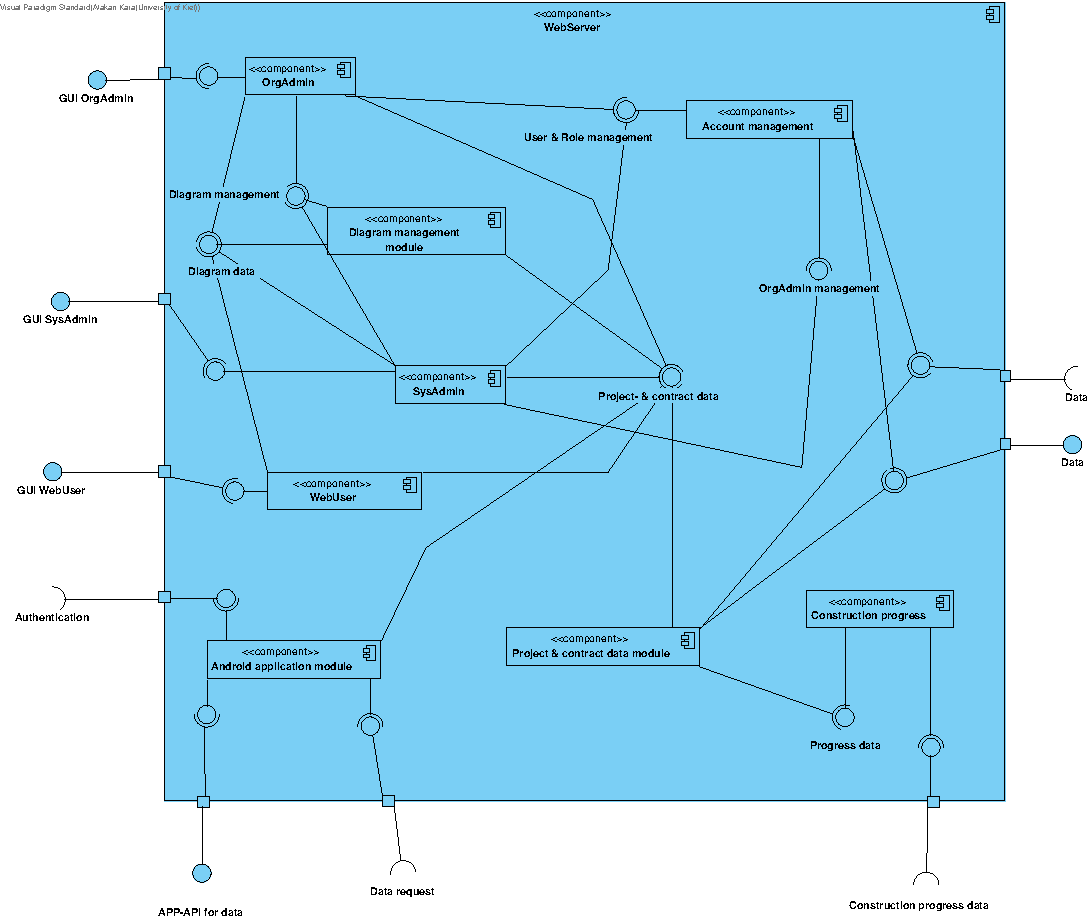
\includegraphics[width=16cm]{img/diagrams/Component-WebServer.pdf}	
	\caption{Komponentendiagramm - WebServer}
	\label{fig:komponentendiagramm-webserver}
\end{figure}

\section{App}

\begin{figure}[H]
	\centering
	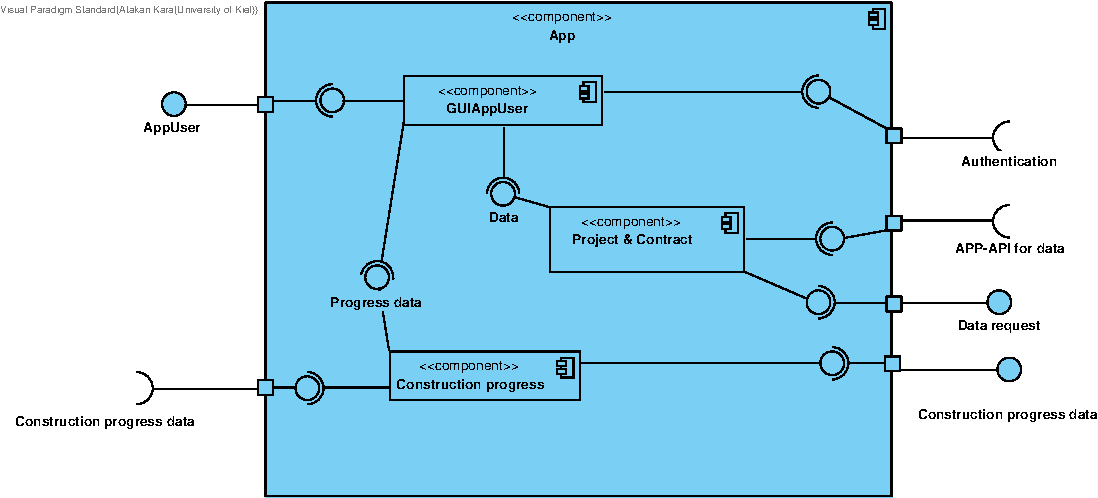
\includegraphics[width=16cm]{img/diagrams/Component-App.pdf}	
	\caption{Komponentendiagramm - App}
	\label{fig:komponentendiagramm-app}
\end{figure}
